% Pascal from Cayley-Bacharach: the cubics AB+CD+EF (blue) and BC+DE+FA (red) meet in A..F and X, Y, Z; the conic plus the line XY passes through 8 of them, hence through Z.
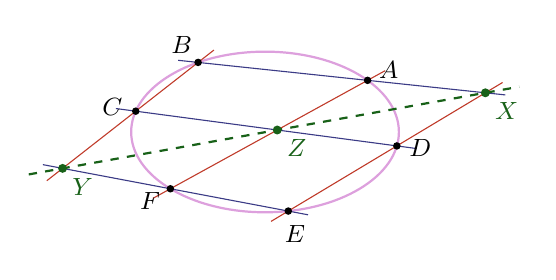
\begin{tikzpicture}[scale=0.85,font=\small]
\draw[Plum,thick] (0,0) ellipse (2.0000 and 1.2000);
\draw[MidnightBlue!85] (3.5905,0.5536) -- (-1.2983,1.0708);
\draw[MidnightBlue!85] (-2.2292,0.3501) -- (2.2670,-0.2479);
\draw[MidnightBlue!85] (0.6421,-1.2375) -- (-3.3194,-0.4881);
\draw[BrickRed!85] (-0.7637,1.2240) -- (-3.2609,-0.7287);
\draw[BrickRed!85] (3.5494,0.7395) -- (0.0900,-1.3361);
\draw[BrickRed!85] (-1.6771,-0.9931) -- (1.7950,0.9159);
\draw[ForestGreen!70!black,thick,dashed] (-3.5299,-0.6342) -- (3.7975,0.6755);
\fill (1.5321,0.7713) circle (1.6pt) node[shift={(0.268,0.135)}] {$A$};
\fill (-1.0000,1.0392) circle (1.6pt) node[shift={(-0.208,0.216)}] {$B$};
\fill (-1.9319,0.3106) circle (1.6pt) node[shift={(-0.296,0.048)}] {$C$};
\fill (1.9696,-0.2084) circle (1.6pt) node[shift={(0.298,-0.032)}] {$D$};
\fill (0.3473,-1.1818) circle (1.6pt) node[shift={(0.085,-0.288)}] {$E$};
\fill (-1.4142,-0.8485) circle (1.6pt) node[shift={(-0.257,-0.154)}] {$F$};
\fill[ForestGreen!70!black] (3.2921,0.5851) circle (1.9pt) node[below right] {$X$};
\fill[ForestGreen!70!black] (-3.0246,-0.5439) circle (1.9pt) node[below right] {$Y$};
\fill[ForestGreen!70!black] (0.1825,0.0293) circle (1.9pt) node[below right] {$Z$};
\end{tikzpicture}
